\documentclass[12pt,aspectratio=169]{beamer}

\usetheme{metropolis}

\definecolor{mDarkBrown}{HTML}{FF5722}
\definecolor{mDarkTeal}{HTML}{263238}
\definecolor{mLightBrown}{HTML}{FF5722}

\usepackage{booktabs}
\usepackage{graphicx}
\usepackage{hyphenat}
\usepackage{multirow}
\usepackage{nicefrac}
\usepackage[normalem]{ulem}

\usepackage{pifont}
\newcommand{\cmark}{\ding{51}}
\newcommand{\xmark}{\ding{55}}

\usepackage{minted}
\usemintedstyle{tango}
\newminted[bash]{bash}{%
    autogobble,
    bgcolor=mDarkTeal!10,
    linenos
}
\newminted[py3]{python}{%
    python3,
    autogobble,
    bgcolor=mDarkTeal!10,
    linenos
}
\newminted[sql]{sql}{%
    autogobble,
    bgcolor=mDarkTeal!10,
    linenos
}

\usepackage{polyglossia}
\setdefaultlanguage[variant=british]{english}
\usepackage[english=british]{csquotes}

\defaultfontfeatures{Ligatures=TeX}
\setmainfont{Lucida Sans OT}
\setsansfont[Scale=MatchLowercase]{Lucida Sans OT}
\setmonofont[Scale=MatchLowercase]{Lucida Console DK}

\usepackage{mathspec}
\setmathsfont(Digits,Latin,Greek)[Numbers={Lining,Proportional}]{Lucida Bright Math OT}

\newcommand{\mat}[1]{\ensuremath{\mathbf{#1}}}

\newcommand{\R}{\ensuremath{\mathbb{R}}}

\newcommand{\E}[1]{\ensuremath{\mathbb{E}\!\left[ #1 \right]}}
\newcommand{\V}[1]{\ensuremath{\mathbb{V}\!\left[ #1 \right]}}
\newcommand{\Prob}[1]{\ensuremath{\Pr\!\left( #1 \right)}}
\newcommand{\Normal}[2]{\ensuremath{\mathcal{N}\!\left( #1, #2 \right)}}
\newcommand{\simiid}{\ensuremath{\overset{\text{\tiny i.i.d.}}{\sim}}}

\DeclareMathOperator{\logit}{logit}

\author{Gianluca Campanella}
\date{}



\title{The Data Science workflow}

\begin{document}

\maketitle

\begin{frame}{High\hyp{}level view}
    \only<1>{%
        \begin{center}
            \large%
            Business goal
            \vfill
            $\downarrow$
            \vfill
            Testable hypothesis
            \vfill
            $\downarrow$
            \vfill
            Experimentation and modelling
        \end{center}}
    \only<2>{%
        \begin{center}
            \large%
            Research question
            \vfill
            $\downarrow$
            \vfill
            Obtain $\ \longleftrightarrow\ $ Explore $\ \longleftrightarrow\ $ Model
            \vfill
            $\downarrow$
            \vfill
            Summarise / Operationalise
        \end{center}}
\end{frame}

\begin{frame}{Time allocation}
    \begin{center}
        \LARGE%
        Which takes longer?
    \end{center}
\end{frame}

\begin{frame}[t]{Define the research question}
    \begin{block}{What to do}
        \begin{itemize}
            \item Identify the problem and why it should be solved
            \item Frame it in the context of data collection
        \end{itemize}
    \end{block}
    \vfill
    \begin{block}{What to ask}
        \begin{itemize}
            \item Which metrics do I need to improve?
            \item Which are possible actions to solve the problem?
            \item What is the benefit of solving the problem?
        \end{itemize}
    \end{block}
\end{frame}

\begin{frame}[t]{Obtain the data}
    \begin{block}{What to do}
        \begin{itemize}
            \item Measure the gap between ideal and available
            \item Think about assumptions and limitations
        \end{itemize}
    \end{block}
    \vfill
    \begin{block}{What to ask}
        \begin{itemize}
            \item Are there enough data?
            \item Are they relevant to the research question?
            \item Can they be trusted?
        \end{itemize}
    \end{block}
\end{frame}

\begin{frame}[t]{Explore the data}
    \begin{block}{What to do}
        \begin{itemize}
            \item Data dictionary and any other documentation
            \item Descriptive statistics and visualisations
        \end{itemize}
    \end{block}
    \vfill
    \begin{block}{What to ask}
        \begin{itemize}
            \item What kind of simple visualisations can I use?
            \item Which data types and distributions?
            \item Are there missing values or outliers?
        \end{itemize}
    \end{block}
\end{frame}

\begin{frame}[t]{Model the data}
    \begin{block}{What to do}
        \begin{itemize}
            \item Model selection and fitting
            \item Focus on inference and/or prediction
        \end{itemize}
    \end{block}
    \vfill
    \begin{block}{What to ask}
        \begin{itemize}
            \item What is an appropriate model for the data?
            \item How can I evaluate model performance?
            \item Can the model be refined?
        \end{itemize}
    \end{block}
\end{frame}

\begin{frame}{Modelling misconceptions}
    Most well\hyp{}executed Data Science projects don't\ldots
    \begin{itemize}
        \item Use complicated tools
        \item Fit complicated models
    \end{itemize}
    \vfill
    Instead, they do\ldots
    \begin{itemize}
        \item Focus on solving the problem
        \item Use appropriate --- not necessarily big! --- data
        \item Use relatively standard models
    \end{itemize}
\end{frame}

{\setbeamertemplate{background}{%
    \rule{0.7\paperwidth}{0pt}%
    \rule{0pt}{\paperheight}%
    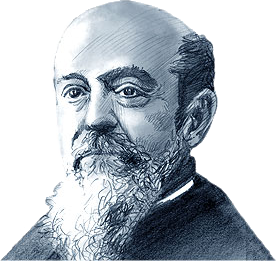
\includegraphics[height=0.6\paperheight]{figures/pareto}}
\begin{frame}{The 80---20 rule of modelling}
    \begin{itemize}
        \item The first reasonable thing you can do goes 80\% of the way
        \item Everything after that is to get the remaining 20\%\ldots \\
              often at additional cost!
    \end{itemize}
    \vfill\pause
    \begin{center}
        \Large%
        Is it worth it?
    \end{center}
\end{frame}}

\begin{frame}{Wait a second\ldots}
    \begin{center}
        \LARGE%
        We are not done yet!
    \end{center}
\end{frame}

\begin{frame}[t]{Summarise the findings}
    \begin{block}{What to do}
        \begin{itemize}
            \item Storytelling and visual aids to interpretation
            \item Communicate assumptions and limitations
        \end{itemize}
    \end{block}
    \vfill
    \begin{block}{What to ask}
        \begin{itemize}
            \item How can I communicate results effectively?
            \item What format should I adopt?
            \item Who are my audience?
        \end{itemize}
    \end{block}
\end{frame}

\begin{frame}[t]{Operationalise}
    \begin{block}{What to do}
        \begin{itemize}
            \item System integration
            \item Monitoring and maintenance
        \end{itemize}
    \end{block}
    \vfill
    \begin{block}{What to ask}
        \begin{itemize}
            \item What (visual) outputs do I care about?
            \item How often does the model need retraining?
            \item Do we need to think about scalability?
        \end{itemize}
    \end{block}
\end{frame}

\end{document}

